% !TEX root = ../main.tex

\chapter{Elliptic curves in Hermes}
\label{OurElliptic}
%% Chapter intro
Elliptic Curve Cryptography (ECC) is, in many ways, the future of public-key cryptography\cite{ECCoverRSA}. The most attractive quality of ECC is the need for smaller keys to achieve the same level of security when compared with RSA. An implementation of ECC will, naturally, take up much more code than RSA, as point-arithmetics need to be implemented, to perform the encryption.

The implementation presented in this chapter is by no means without flaws, but point-arithmetic operations have been successfully implemented, and improvements are suggested for all of the flaws in the implementation.  

The implementation is documented with unit-tests, verifying the results of the implementation against s small elliptic curve python library.  

\section{User Guide}
%%%%%%%%%%%%%%%%%%%%%%% Finish writing this. Maybe refer to the Hermes repo, for an explanation on how to make a compiler, before calling the Makefile.
The implementation of Elliptic Curve Cryptography can be found in the \texttt{elliptic.hms} file, located in the \texttt{src.zip} folder. Within the folder is also found a \texttt{Makefile}, which allows for easy compilation of the program. Simply do a:
\begin{lstlisting}[language=C]
  $ make elliptic
\end{lstlisting}%$
and it should compile, first to \texttt{C}-code, and then compile that generated code using \texttt{GCC}. This requires the Hermes compiler to be located in the same folder as the \texttt{Makefile} and \texttt{elliptic.hms}. For instructions on how to build the compiler, see Section \ref{HC}.

Running the code is simple as well\footnote{See section \ref{RunTest} for an explanation on how to run the tests.}, just run the command-line:
\begin{lstlisting}[language=C]
  $ ./elliptic
\end{lstlisting}%$
A prompt should then appear, taking two 32-bit unsigned integers, after which the encryption and subsequent decryption should begin. 

\section{Analysis}
\label{ellipticAnalysis}
%%%%%% Mere der kan snakkes om: 
%%%%%% - Hvad sker der i den faktiske kryptering/dekryptering? Måske ikke så relevant, da dette bør være dækket i background.
A cryptographic scheme that uses elliptic curves consists of a few elements:
\begin{itemize}
\item Some elliptic curve arithmetic: This is used both to generate keys, but also to establish a shared secret.
\item Some synchronous encryption scheme: Any non-trivial encryption algorithm will do the trick, as the safety lies in the key.
\item A key derivation function: Since most symmetric cryptography schemes do not use points on a curve as keys (which is what is established as a shared secret with ECC), a function is needed to derive a key from such a point. 
  %use numbers as keys, the shared secret, generated using elliptic curve arithmetic (a point on the curve), does not work as a key. Therefore a function is needed to derive a key from a point on the curve.
\end{itemize}
Not all of these elements are particularly interesting, but they must all be considered for an implementation to function. There is also the issue of how to represent the actual curve, points, point-at-infinity, etc. This is left for section \ref{ellipticDesign} - Design. 
\subsection{Elliptic Curve Arithmetic Functions}
Recall from section \ref{elliptic} the arithmetic operations that can be performed on points on an elliptic curve:
\begin{itemize}
\item Point-addition.
\item Point-doubling.
\item Point-multiplication.
\end{itemize}
The operations are the main body of what needs to be implemented. Point multiplication is, intuitively, simply several additions, much like in regular algebra. Furthermore, point-doubling can be done by adding a point to itself, and so both of these functions make use of point-addition to some extend.

When attempting to implement these function reversibly, however, it makes sense to think of point-addition and point-doubling as separate functions, as one is significantly more complicated to reverse than the other. Geometrically, it is not hard to see why this is the case, as finding the slope of the line that intersects the curve at some point and exactly one other point, should sound more convoluted than drawing a line through two points, and finding the third point where it intersects the curve. This will be explored in more detail in Section \ref{In-Place}

There is also the matter of handling the point-at-infinity. This can be fairly simple in a non-reversible language, but with the restrictions of Hermes, it becomes non-trivial. It can be handled with a bunch of \texttt{if}-statements, but where a non-reversible language can get away with something as simple as:
\begin{verbatim}
if (Px==Qx) return infinity;
\end{verbatim}
this becomes more convoluted in Hermes. The precise way to handle this is still with \texttt{if}-statements, but as can be seen in section \ref{ellipticImplementation}, the way Hermes handles \texttt{if}-statements makes it a bit more complex. 

The only difference, in calculating the coordinates for the result of a point-addition and a point-doubling, is the formula for computing $\lambda$. It is possible to have a single function that checks if the two points are the same, but there are once again some complications with reversibility. This method assumes that there will always be two points, meaning that it is not possible to pass a single point and get the $\lambda$ for doubling that point. Because of this, it makes sense to maintain two separate functions for calculating $\lambda$, but as can be seen in section \ref{ellipticImplementation}, it is beneficial to have the function for calculating $\lambda$ for separate points be able to detect if those two points have the same coordinates.

Multiplication can, as mentioned above, be implemented as a series of additions. This will be the case in this implementation, due implementation problems with point-doubling, but it is possible to be smarter about multiplication. Although many algorithms exist for efficient multiplication, not all are useful when applied to elliptic curves, and even fewer when implementing them in Hermes. The main issue with implementing a more efficient algorithm would be the restrictions on \texttt{for}-loops in Hermes. Since these can only loop over constants, it is not possible to do:
\begin{verbatim}
  mult(x,y)
    res = x
    for (i=0;i<y;i++)
      res += x
    return res
\end{verbatim}
Instead, the options for looping are to either loop over the largest possible value for $y$ (which, when keys grow to useful sizes, becomes impractical) or to loop over the size of the representation of $y$. An algorithm that implements that second option can be seen in Figure \ref{mult}.
\begin{figure} 
\begin{verbatim}
    mult(u32 P[2], u32 R[2], u32 k){
      u32 tmp[2], sum[2];
      tmp[0] += P[0];
      tmp[1] += P[1];
    
      for (i=0;32){
        if (k&(1<<i)) call add(tmp, sum);
        call double(tmp);
        i++;
      }
      // Clear local variables. 
      sum[0] <-> R[0];
      sum[1] <-> R[1];
      
    }
\end{verbatim}
  \caption{An implementation of \texttt{mult} in Hermes.}
  \label{mult}
\end{figure}

This is an incomplete algorithm for several reasons. It is missing certain parameters, such as the $a$-coefficient of the curve, which is needed for doubling a point. This parameter should be passed to \texttt{double}, for it to work properly. The variable \texttt{tmp} also needs to be cleared before execution. How to clear this variable will depend on the implementation of double. There are likely to be other errors in it, as this has not been possible to test.

This multiplication algorithm calls a \texttt{double} function, that works in-place. The issues with implementing such a function will be mentioned in Section \ref{In-Place}, and are the main reasons why a less efficient multiplication has to be used. 
\newpage
\subsection{Symmetric Encryption}
Elliptic curve cryptosystems make use of symmetric encryption. This symmetric encryption plays a role in the strength of the elliptic curve crypto scheme, but the asymmetric part of the scheme has nothing to do with it. Thus, it is not of significant interest here, to analyze different symmetric encryption schemes, and find the one that fits best.

Instead, a more pragmatic approach has been taken, and the \textit{Tiny Encryption Algorithm} was chosen from the existing Hermes implementations from \cite{PSI19}. 
\subsection{Key Derivation Function}
As mentioned above, points are not normally used as keys for encryption schemes. This is indeed the case for \texttt{TEA}, and so a function is needed to derive a key from a point on the curve. Since the point is secret, there are not any requirements for such a function, apart from having to satisfy the type of the key used in \texttt{TEA}.

To produce a key that is useful in \texttt{TEA} it suffices to generate the key based on a mishmash of logical operations on the coordinates of the point. More advanced functions could be used, but as the strength of the scheme lies in generating the point, that would yield no real advantage over this simple approach. 
\section{Design}
\label{ellipticDesign}
%%%%%% Mere der kan snakkes om:
%%%%%% - 
In designing the solution for this project, the main concerns have been to adapt algorithms and procedures to be reversible. As several versions exist of Hermes, there is also a choice to be made there.

\subsection{Choosing a Hermes Version}
Two main implementations of Hermes exist, Hermes and Hermes2. When considering which to implement the solution in, the newest version, i.e. Hermes2, is the obvious first consideration. Hermes2 introduces \texttt{Public}/\texttt{Private} types. The motivation behind making certain variables public is to ease restrictions on loop bounds\cite{Hermes2}, and on the language in general. This might seem like an attractive feature, considering the number of issues with looping in the implementation (see section \ref{Problems}), but since these loops are done over keys and other shared secrets, there would be nothing to gain from this.

The original Hermes is a syntactically simpler language, although it is more restrictive. There exists a cross-compiler from Hermes\footnote{This compiler is not compatible with Hermes2.} to \texttt{C}, which means easy compilation, execution, verification and debugging (since GDB\footnote{https://www.gnu.org/software/gdb/} can be used to debug the compiled \texttt{C} code).

This simplicity of Hermes(1) as well as the ease of use is what made the original Hermes the language of choice for this solution. 

\subsubsection{Implications of \texttt{C} as Target Language}
For the most part, operations in Hermes are fairly basic, and as such, the implementations of them in \texttt{C} are as one would expect. Integer addition, subtraction, multiplication, and division, as well as binary logical operators, are straight forward. The one operator, that demands care when using, is the modulo operation. As this solution is heavily reliant on modulo arithmetic, to perform the elliptic curve operations within a prime field, this needs to be carefully considered. In the documentation for \texttt{C}, the modulus is described as "Modular division returns the remainder produced after performing integer division on the two operands"\footnote{https://www.gnu.org/software/gnu-c-manual/gnu-c-manual.html}. This remainder is not the same as finite field modulo, as negative remainders fall outside of the field.

This is no big problem and it can be solved by replacing all modulo operations as such:
$$
\mathtt{(exp)\%p;} \longrightarrow \mathtt{(((exp)\%p)+p)\%p;}
$$
Performing modular operations like this ensures that negative numbers get "flipped" inside of the prime field while leaving numbers that are already within the field unchanged. 


\subsection{Representation of Curves and Points}
Since Hermes does not allow the creation of structs and does not have other types than integers and arrays, representing curves and points on them must be done using only these. The simplest of these to represent is the curve itself. Since the only aspect of the curve that is of interest when calculating new points is the $a$-coefficient of the curve, it can be represented as a single integer number. Since the curve is defined in a finite field, this field must also be represented. For the sake of simplicity, the solution implements prime fields rather than extension fields. There is no other motivation behind than that of making it easier to implement. This choice means that the field can be represented as a single integer and that operations simply need to be performed modulo that integer.

Points are also fairly simple to represent, but a few options are available. One option would be to simply keep track of the $x$- and $y$-coordinates separately as integer numbers. This is not an uncommon practice, as they are needed in different places in the computations. The drawback of such a representation is the verbosity of function parameters.

Another option, which is the one chosen for this implementation, is to represent numbers as arrays with 2 elements, with the first element being the $x$-coordinate and the second being the $y$-coordinate. The array still contains integers, so the representation of the coordinates remains unchanged, but this provides a more compact option for passing points as parameters. One unforeseen drawback from this design choice, combined with the choice of using an older version of Hermes, is the fact that the compiler for Hermes does not allow for updating an element of an array with other elements of the same array. This should be possible, according to \cite{PSI19}, as each element is a separate variable. This does not hinder the implementation, but it does make for some longer than necessary expressions at times (e.g. the $x$-coordinate of the point that is being calculated is a part of the calculation for the $y$-coordinate, so the expression of the $x$-coordinate must be used instead of just the first element of the array).

One last thing to consider is the point at infinity. This must be the additive inverse for the elliptic curve, so choosing a representation is not trivial. One might be tempted to use the point $\{0,0\}$(as $0$ is the additive inverse in regular arithmetic), but as this can be a valid point on the curve, it is not a possibility. As the point of infinity has to be handled explicitly, any point would work in theory, provided the point cannot appear on the curve. Since the curve is represented in a finite field (in this particular case a prime field) with base $p$, the point $\{p,p\}$ is a suitable candidate for representing the point of infinity. This makes the implementation adjustable to different curves while providing an easy-to-handle point at infinity.

\subsection{Key Generation}
While attempting to implement RSA in Hermes, the focus was deliberately shifted away from key generation, as it is an entirely different procedure than that of the actual encryption/decryption. While the focus is still not to implement key generation in ECC, the encryption, decryption, and key generation of ECC are much more interrelated than that of RSA. Private keys are randomly chosen numbers, which has not been attempted in Hermes, but generating a public key from the privately known number is a simple point-multiplication.

Because of this, it is more convenient to generate the keys in the function that runs the encryption/decryption, rather than decide on a key-pair beforehand, and give those as an input to the program. The private key could be entered by the user when running the program, but for simplicity, it is just hard-coded where decryption and key generation happens. 

\subsection{Designing Point-Arithmetic Functions}
%%%%%% - Initial design: out-of-place
When designing the actual point-arithmetic functions, initially they were made out-of-place, i.e. two points were added together and stored in a third point, or one point was doubled and stored in a second point. This is a simple design, but it seems reasonable, as ECC generates new points, rather than updating existing ones. This means that both point-addition and point-doubling take an empty point, $R=\{0,0\}$, as input, to store their results in. 
%The functions (both addition and doubling) then take the points to have the operation performed on, as well as a point that is assumed to be $R=\{0,0\}$.

Such functions are slightly different from what one might expect from elliptic curve arithmetic functions, in that their inverse is not what would be arithmetically pleasant for it to be. Uncalling such a point addition would not be the same as subtracting one point from another, but rather it would just clear the result. This can be quite handy for clearing local variables, as will be seen in the implementation.

The formulae for calculating the $\lambda$ used in computing the coordinates for the new point are designed in a similar manner. This way it is possible to define a local variable \texttt{s}, compute $\lambda$ in \texttt{s} by calling \texttt{calcS} and after calculating the new point, \texttt{s} can be cleared again by uncalling \texttt{calcS}. 


\subsection{Operations In-Place}
\label{In-Place}
%%%%%% - Add kan laves in-place (graf der viser hvordan vi adder in place.)
Although these out-of-place functions calculate the new point perfectly well, they are not quite what is needed. As mentioned in the previous section, their inverses are not exactly the arithmetically inverted function, but rather a clearing of the result. The trouble in implementing these functions in-place was hinted at in the analysis (Section \ref{ellipticAnalysis}).

Starting with point-addition, it is not too troublesome to perform this operation in-place. Recall the geometry of point-addition of two points $P$ and $Q$:
\begin{figure}[H]
    \centering
    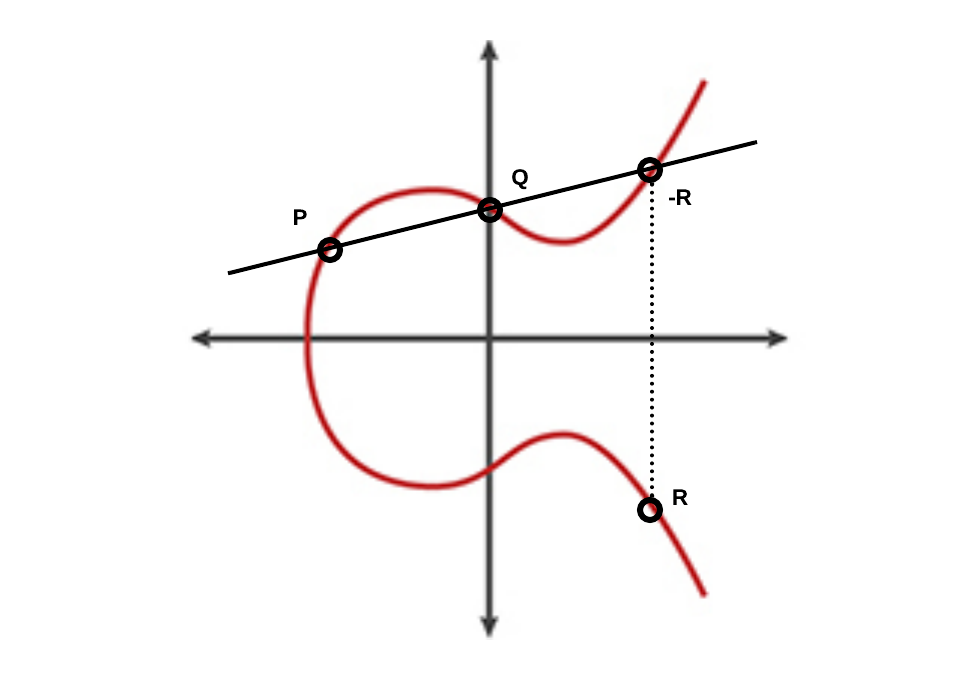
\includegraphics[width=0.5\textwidth]{figures/EcAdd}
    \caption{Point-addition on an elliptic curve.}
\end{figure}
The general idea for an algorithm that adds \texttt{P} to \texttt{Q}, in \texttt{Q}, is:
\begin{enumerate}[1)]
\item Calculate \texttt{-R} in a temporary variable.
\item Swap the values of \texttt{Q} and that temporary variable.
\item Clear the temporary variable, which is now \texttt{-(P+Q)} with \texttt{Q} holding the value for \texttt{-R}.
\item Flip \texttt{Q} to the other side of the curve, which is as simple as negating the $y$-coordinate.
\end{enumerate}
There are other ways to calculate the old point in order to clear the variable, but this is an easilly understandable method, and the example from above can now be shown, using this method:
\begin{figure}[H]
    \centering
    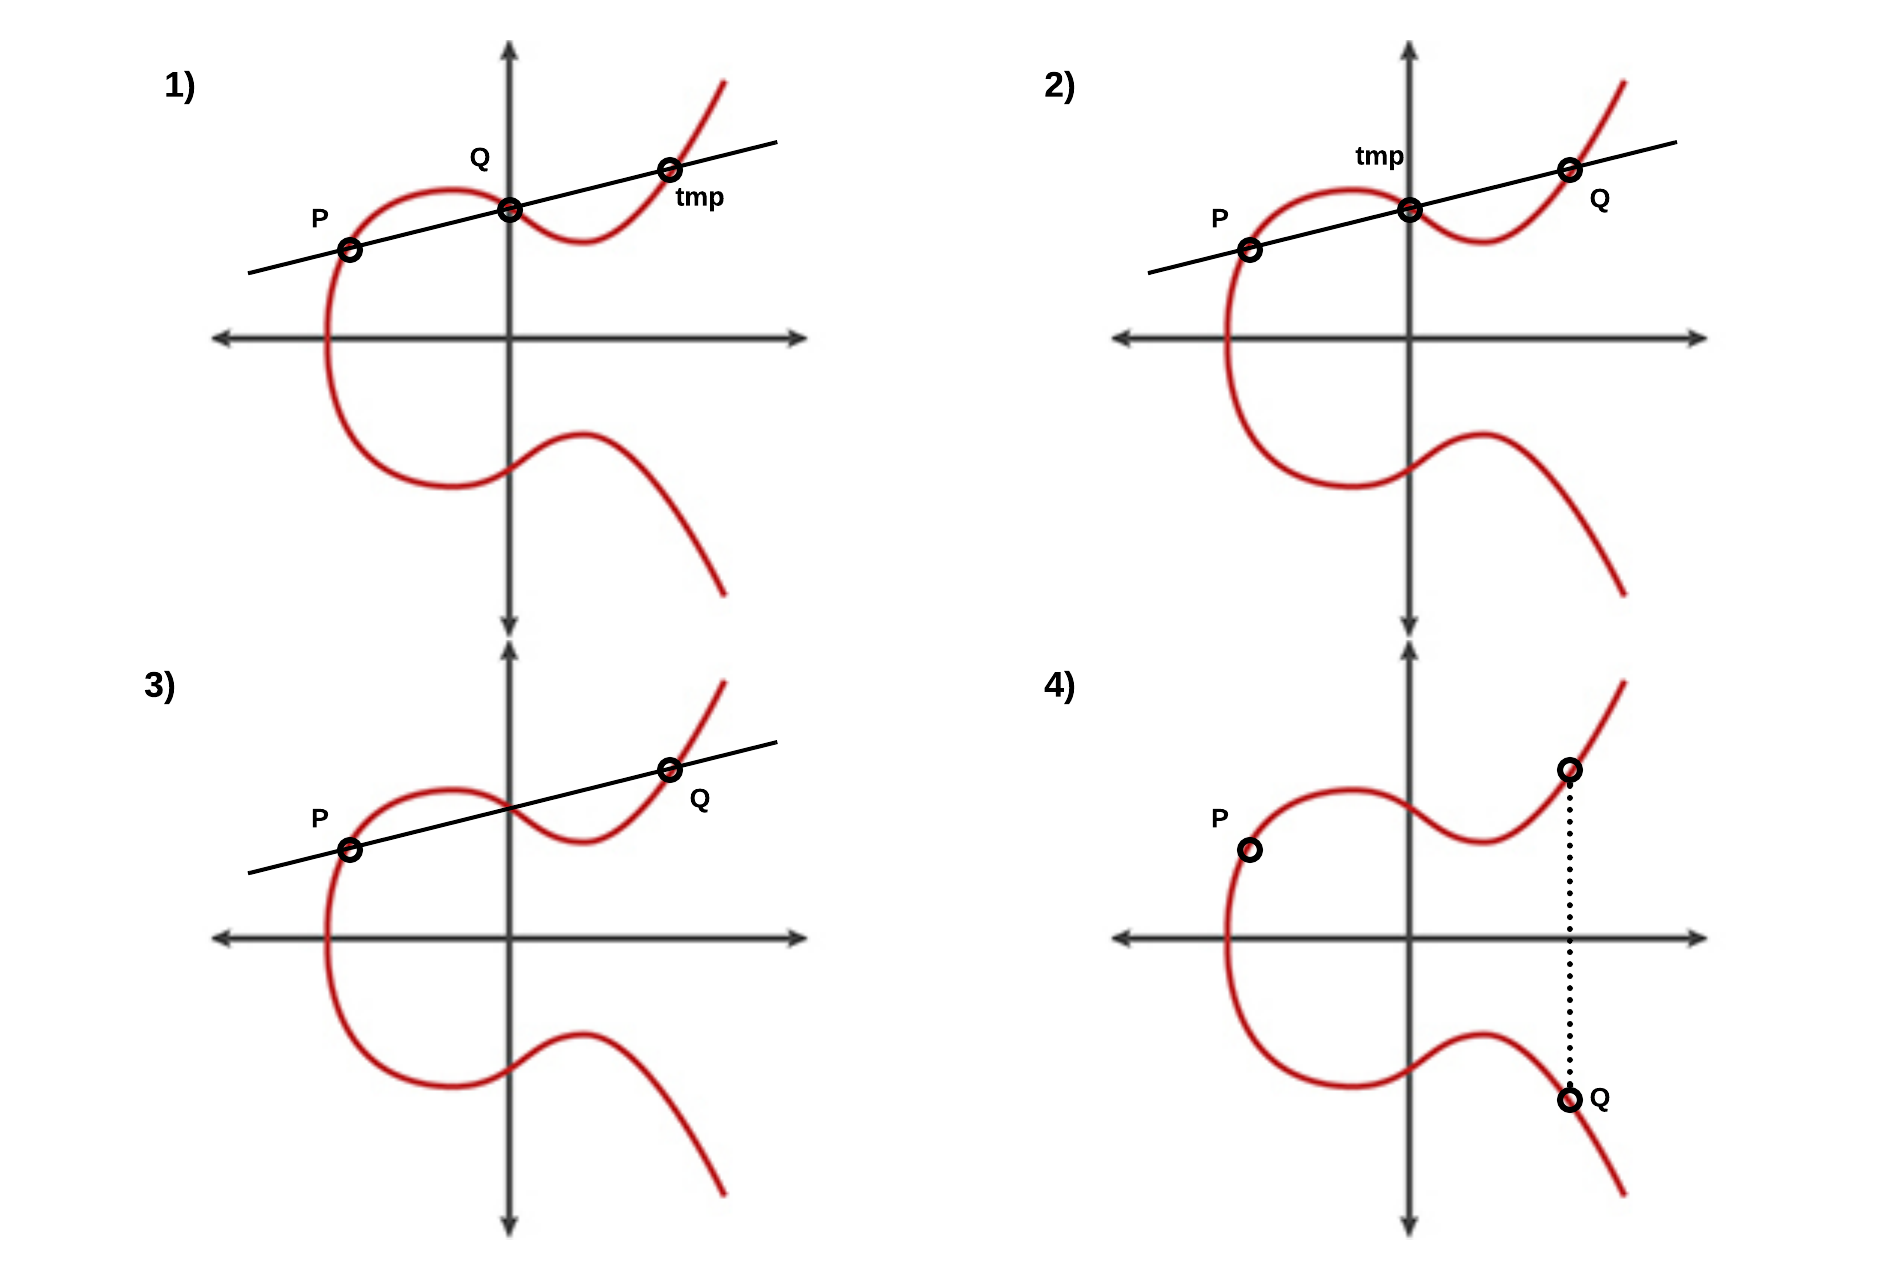
\includegraphics[width=0.8\textwidth]{figures/InPlaceAdd}
    \caption{Step-by-step example of the in-place point-addition algorithm.}
\end{figure}

Unfortunately, point-doubling is not nearly as convenient to implement. To understand why this is problematic, consider implementing the inverse function: point-halving. Attempting to backtrace a point doubling, initially flipping the point is no problem. However, this is where the problems do arise. Trying, from one point, to find the line, which intersects that point and exactly one other point on the curve, essentially boils down to solving a system of 3 equations\cite{Halving}. The subject of point-halving is well beyond the scope of this project, and so an out-of-place algorithm for point-doubling will have to suffice. 
\subsection{Multiplication}
%% So what have we actually done to multiply.
In Section \ref{ellipticAnalysis} a method for multiplying is mentioned, which used both doubling and addition to perform the multiplication. This implementation loops over the binary representation of the number that is being multiplied by, and so is a decent method for implementing elliptic curve point-multiplication. This method requires an in-place point doubling, however, and so the \texttt{double} which has been implemented and will be presented in Section \ref{ellipticImplementation} does not allow for this.

So what options are available? Due to the previously mentioned restrictions on loops in Hermes, it is not possible to loop until the number that is being multiplied by, adding the base number every time.

Looping, until the maximum size of the number that is being multiplied by, seems the only remaining option. This is not a good solution, by any stretch of the imagination, but it is the best that can be done at the current. The issues with the implementation of this multiplication are discussed in Section \ref{Problems}. 

\section{Implementation}
\label{ellipticImplementation}
At the core of Elliptic Curve Cryptography is point-addition. This is also the case for this implementation, as point-addition is where the majority of the work is done. Thus the function \texttt{add} will be a sensible place to begin exploring the code.
\subsection{Point-Addition}
\label{PointAdd}
\begin{figure}[H]
\begin{Verbatim}
// Point addition in place. Saves result in Q. 
add(i32 P[2], i32 Q[2], i32 a, i32 cond, i32 p){
  i32 s, infP, infQ, noInf, infRes;
  i32 tmp[2];
  
  //Checking conditions for point-at-infinity. 
  if (cond) infP += (P[0]==p)&(P[1]==p);
  if (cond) infQ += (Q[0]==p)&(Q[1]==p);
  if (cond) infRes += (P[0]==Q[0])&(P[1]!=Q[1]);
  if (cond) noInf += (infP==0)&(infQ==0)&(infRes==0);
  
  //// Point addition when the points are distinct and neither is infinity:
  call calcS(s, P, Q, a, p);
  if (cond&noInf) tmp[0] += (((s*s-P[0]-Q[0])%p)+p)%p;
  if (cond&noInf) tmp[1] += (((((P[1]-s*(P[0]-((s*s-P[0]-Q[0])%p)+p)%p)))%p)+p)%p;    
  if (cond&noInf) Q[0] <-> tmp[0];
  if (cond&noInf) Q[1] <-> tmp[1];
  if (cond&noInf) tmp[0] -= (((s*s-P[0]-Q[0])%p)+p)%p;
  if (cond&noInf) tmp[1] -= (((P[1]-s*(P[0]-((((s*s-P[0]-Q[0])%p)+p)%p)))%p)+p)%p;  
  uncall calcS(s, P, Q, a, p);                
  if (cond&noInf) tmp[1] += (((-Q[1])%p)+p)%p;
  if (cond&noInf) Q[1] <-> tmp[1];            
  if (cond&noInf) tmp[1] -= (((-Q[1])%p)+p)%p;
  
  //// Point addition when Q is infinity:
  if (cond&infQ) Q[0] -= p;
  if (cond&infQ) Q[1] -= p;
  if (cond&infQ) Q[0] += P[0];
  if (cond&infQ) Q[1] += P[1];
  
  //// If the two points have the same X-coordinate:
  if (cond&infRes) Q[0] -= P[0];
  if (cond&infRes) Q[1] -= (((-P[1])%p)+p)%p;
  if (cond&infRes) Q[0] += p;
  if (cond&infRes) Q[1] += p;
  
  // Clear conditionals. 
  if (cond) noInf -= (infP==0)&(infQ==0)&(infRes==0);   
  if (cond) infP -= (P[0]==p)&(P[1]==p);
  if (cond) infRes -= (Q[0]==p)&(Q[1]==p);
  if (cond) infQ -= (Q[0]==P[0])&(Q[1]==P[1]);
}
\end{Verbatim}
\caption{Hermes implementation of elliptic curve point addition.}
\end{figure}
\noindent Comments had to be removed from the code, to fit the page. A lot is going on here, so consider the 4 cases that addition must handle:
\begin{enumerate}[i)]
\item The two points are distinct points on the curve, neither is the point-at-infinity, and their sum is not infinity either. This case is handled in the manner described in Section \ref{In-Place}.
\item The point that is being added onto is the point-at-infinity. Since the sum of $\mathcal{O}$ and any other point results in that other point, this case needs to change the point \texttt{Q} (which is infinity) to be the point \texttt{P}, since the function saves the result in the second point. 
\item The points have the same $x$-coordinate, and thus their sum is the point-at-infinity. This would not be handled by the arithmetic expression for computing coordinates, and so it needs to be handled explicitly by first clearing the point \texttt{Q} and the setting it to be $\{p,p\}$.
\item The point that is being added is the point-at-infinity. Handling this case is trivial, with the current design, as nothing needs to be done here.
\end{enumerate}
Several conditions are checked at the beginning of the function and are used for handling these cases, but one condition is also passed to the function as an argument. This condition is needed because of the way the addition is called. In the multiplication that will be presented below, \texttt{add} should, ideally, have been called conditionally (i.e. \texttt{if(condition) call add();}), but Hermes does not allow for that. Thus, as a workaround, the function takes the condition as an argument, and performs all updates and swaps conditionally.\\

To calculate the $\lambda$ needed for the coordinates of the new point, \texttt{add} calls a function \texttt{calcS}. This function needs to be a bit more complicated than just calculating:
\[s=\frac{P_y-Q_y}{P_x-Q_x}\]
because of the way the curve loops around, after adding the generator point to itself $p$ times ($p$ being the base of the prime field $\mathcal{F}_p$ that the curve is defined on). On a curve with a generator $G$ that can reach all points on the curve, the point $pG$ will end up being $-G$. Therefore, with the method used to add in-place, \texttt{calcS} has to check if the two points have the same coordinates, in order to always be able to clear the variable \texttt{s}.
\begin{figure}[H]
\begin{Verbatim}
// Assuming s=0 when calling, and resetting s=0 by uncalling. 
// s = (yP - yQ) / (xP - xQ) hvis P != Q.
// s = (3xP**2 + a) / (2yP ) hvis P == Q.
calcS(i32 s, i32 P[2], i32 Q[2], i32 a, i32 p){
  i32 tmp1, tmp2, same, distinct;              // Defining variables.
  
  same += (P[0]==Q[0])&(P[1]==Q[1]);           // Checking if points are the same.
  distinct += (P[0]!=Q[0])|(P[1]!=Q[1]);       // Checking if points are distinct.
  if (distinct) tmp1 += (((P[1]-Q[1])%p)+p)%p; // Dividend for distinct points. 
  if (distinct) tmp2 += (((P[0]-Q[0])%p)+p)%p; // Divisor for distinct points. 
  if (same) tmp1 += (((3*P[0]*P[0]+a)%p)+p)%p; // Dividend for equal points. 
  if (same) tmp2 += (((2*P[1])%p)+p)%p;        // Divisor for equal points. 
  
  call gfDiv(tmp1,tmp2,p,s);                   // Galois field division. 
  
  // Resetting variables to 0. 
  if (distinct) tmp1 -= (((P[1]-Q[1])%p)+p)%p; 
  if (distinct) tmp2 -= (((P[0]-Q[0])%p)+p)%p; 
  if (same) tmp1 -= (((3*P[0]*P[0]+a)%p)+p)%p;
  if (same) tmp2 -= (((2*P[1])%p)+p)%p; 
  same -= (P[0]==Q[0])&(P[1]==Q[1]);
  distinct -= (P[0]!=Q[0])|(P[1]!=Q[1]);
}
\end{Verbatim}
\caption{Function for calculating $\lambda$.}
\end{figure}

To always perform the division correctly, a helper function is needed for a Galois field division. This function simply checks all numbers in the field to see if they fit as a solution to:
\[\frac{x}{y}~mod~p=z~~~~iff.~~~~z*y~mod~p=x\]
Because of the restrictions on loops in Hermes, this function is hard-coded to fit the field $GF(17)$. For a more general approach, Hermes2 and its type system of public and private variables could be useful. Since the field that is used for the encryption is no secret, this function could be given a public $p$ to loop over. This is an optimization, however, and not a major concern for this implementation.
\subsection{Point-Doubling}
The observant reader might be wondering, why an explicit doubling method is at all needed when the addition can handle points with the same coordinates. And it is indeed possible to implement doubling by taking a copy of the point to be doubled and adding these two points together. However, due to the complexity of \texttt{add}, it seems reasonable to attempt to call it as seldom as possible.

When doubling is implemented out of place, i.e. with a destination point (point in which to put the result) as input, the function is quite simple:
\begin{figure}[H]
\begin{Verbatim}
// Doubles a point.
double(i32 P[2], i32 R[2], i32 a, i32 p){ 
  i32 s;
  call calcSD(s,P,a,p);
  R[0] += (((s*s - 2*P[0])%p)+p)%p;
  R[1] += ((((-P[1])+s*(P[0]-((((s*s - 2*P[0])%p)+p)%p)))%p)+p)%p;
  uncall calcSD(s,P,a,p);
}
\end{Verbatim}
\caption{Out-of-Place implementation of point-doubling..}
\end{figure}
Notice how the function does not call \texttt{calcS}, but instead calls \texttt{calcSD}. This is just a function that computes the same result at \texttt{calcS} would, given two identical points, but without the need for two points as input.

\subsection{Encryption/Decryption}
Encryption and decryption have been implemented per the Elliptic Curve Integrated Encryption Scheme\footnote{https://en.wikipedia.org/wiki/Integrated\_Encryption\_Scheme}. On a predetermined curve and field, \underline{encryption} is:
\begin{enumerate}[1)]
\item A point $S=r\cdot Q$ is generated, where $Q$ is the public key of the recipient, and $r$ is a random number. 
\item A point $R=r\cdot G$ is generated, where $G$ is the generator point of the curve.
\item A key is derived from the point $S$.
\item The message is encrypted using the key and sent to the recipient along with the point $R$.
\end{enumerate}
When receiving the encrypted message and the point $R$, \underline{decryption} is done by:
\begin{enumerate}[1)]
\item A point $S=d\cdot R$ is generated, where $R$ is the number received from the sender, and $d$ is the private key of the recipient.
\item A key is derived from the point $S$.
\item The message is decrypted using the key.
\end{enumerate}
Apart from these fundamental steps, the reversible functions also need to clear variables, etc., but this is the core functionality. The point $R$ is passed to both encryption and decryption as an argument and is not cleared by either. This is not an issue, as it is information to be sent in-the-clear, so in the implementation, it is cleared by writing it out to the terminal. 
\subsection{Problems and Shortcomings}
\label{Problems}
%%%%%% - Snak om problemerne med implementationen.
The biggest issue with this implementation is the method for performing point-multiplication. There are two major issues with the current implementation, which are related to each other:
\begin{itemize}
\item Either this becomes unbelievably slow, to the point where it is not useful.
\item Or the number to multiply with has to be limited on its size, meaning smaller key-sizes and thus less secure encryption.
\end{itemize}
As the implementation stands at the moment, with an 8-bit signed integer as the number that is received by the multiplication, a brute force attempt at breaking the encryption would not take more than at most 127 iterations to crack.

The first problem is just as spectacularly bad in the current implementation, as can be demonstrated by adjusting the size of the keys. In modern encryption schemes, keys with triple-digit bit-representations are not uncommon, unfortunately, Hermes does not allow for such large types. Luckily, a 32 bit signed integer works just fine to demonstrate the embarrassing run time of \texttt{mult}. Below can be seen a timed run of a single multiplication test, where the loop in \texttt{mult} has been changed to cap at $2147483647$ (the max value of a 32-bit signed integer):
\begin{figure}[H]
    \centering
    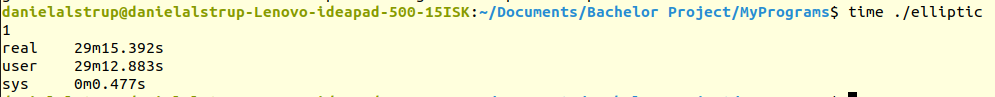
\includegraphics[width=1.0\textwidth]{figures/timeElliptic}
    \caption{Timed execution of a single elliptic point-multiplication.}
\end{figure}
\noindent The underlying problem with the multiplication is the \texttt{double}-function, covered in Section \ref{In-Place}, where a possible improvement was also presented. \\

The Galois field division is also lacking in generality, which is also in part due to the looping in Hermes. It has, however, already been hinted at, that this specific problem has a much simpler solution to it: use Hermes2 and implement it with a public variable $p$, so that the function can loop over the variable. 
\section{Testing}
To test the implementation, the results of operations are compared to the results from an elliptic curve Python library \texttt{tinyec}\footnote{https://github.com/alexmgr/tinyec}. As the tests will not be covering the efficiency and safety of the implementation, there is no need for state-of-the-art libraries, and a simple-to-use library will suit these functional tests much better.

\subsection{A Test Setup in Hermes}
Due to the many restrictions of Hermes, a setup for unit-testing needs to obey these restrictions as well. Luckily, many of the issues with zeroing variables are made much easier, since writing the results of the tests out will clear the variables that are printed. Also, the fact that variables need to be zeroed can somewhat function as a means to check the results. If by subtracting the expected value from the variable, it is not returned to zero, then it did not have the expected value.

This method of testing can, however, become very messy, with error messages all over the screen, whenever the functions do not work as intended. Therefore, the results of each test are saved in an array, such that the $i^{th}$ index of the array holds the result of the $i^{th}$ test. That way, after running all the tests, the array can be printed, element-by-element, and if the $j^{th}$ number printed out is a $0$, then the corresponding test can be immediately found.

\subsection{Writing Tests}
The writing of tests also needs a bit of care. Hermes only allows the scope of a function to be its arguments and whatever variables are defined within it. This means, that each test needs to set up its curve and prime field, before performing any operations on these. It would be possible to have one function perform several operations, but that would be against the principles of unit-testing (isolating units and testing them independently).

This means, that the tests are rather verbose, and many are similar in design. The design of the tests could perhaps be more elegant, but the energy seemed better spent elsewhere.
\\

When it comes to the actual contents of the tests, the small elliptic curve, that is used in the implementation, allows for quite a simple and complete method for testing. Since the order of the selected curve is $n=18$ with a cofactor $h=1$\cite{ECmod17}, it is possible to reach all points on the curve, starting from the generator point. Thus, with a finite amount of tests (17 to be exact), it is possible to verify if multiplication handles all possible special cases. 

Tests designed to fail, such as performing addition with points that are not on the curve, do not make much sense, as it is not feasible to end up with a point outside of the curve, provided multiplication can get around the entire curve without issues.

Naturally, a few tests to verify the functionality of addition and doubling are sensible to include, but as these are also part of multiplication, they will be thoroughly tried in those tests as well.

Finally, some integration tests of the general encryption and decryption are included as well, running the scheme with varying keys.   
\subsection{Running Tests}
\label{RunTest}
The test suite consists of a total of 26 tests, ranging from unit tests of a single addition to integration tests of encryption and decryption. The full test-suite is included in the source code in the \texttt{src.zip} folder, and can be run by uncommenting the \texttt{//call runTests();} line in the \texttt{main()}. If only the tests should be run, the line with \texttt{call runCrypt();} needs to be uncommented. 

The tests have been performed on a Lenovo Ideapad 500-15ISK, with an Ubuntu 20.04 distribution as OS. All tests are successful, as seen in the screenshot in the appendix, Figure \ref{fig:ECCTest}. As mentioned above, however, this is not a test of the quality of the solution, only of the correctness of it. The issues discussed in Section \ref{Problems} are not inconsequential because the tests pass, but the basic functionality of elliptic curve arithmetics appears to work as intended. 